\section{Resultados}
\label{sec:resultados}

A Figura~\ref{fig:regressao} ilustra um conjunto de dados simulado a
partir da Equação~\eqref{eq:regressao}, com $\beta_0 = 2{,}0$ e
$\beta_1 = 1{,}5$, junto da reta ajustada.

\begin{figure}[h]
    \centering
    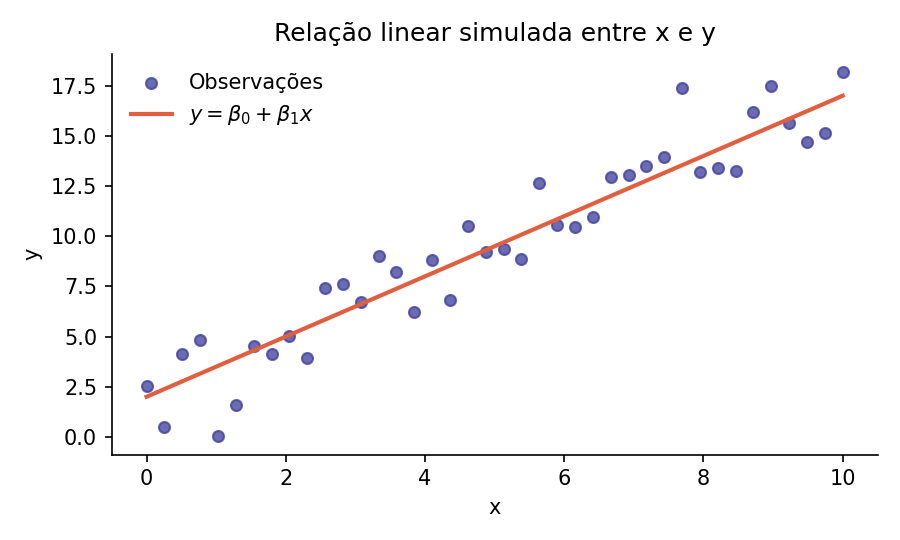
\includegraphics[width=0.75\linewidth]{figura.png}
    \caption{Dados simulados e reta de regressão ajustada.}
    \label{fig:regressao}
\end{figure}

Como esperado, os pontos se distribuem em torno da reta, com dispersão
compatível com a variância do erro $\sigma^2$ definida em cada
experimento (Tabela~\ref{tab:configuracoes}).

\section{Conclusão}
\label{sec:conclusao}

Este exemplo mostrou como organizar um projeto com múltiplos arquivos
\texttt{.tex}, equações numeradas e referenciadas, tabelas, figuras e
citações bibliográficas --- os blocos básicos para escrever um trabalho
acadêmico completo neste editor.
